\chapter{Experiment} \label{cpt-experiment}

When considering occlusion culling algorithms that can be used in a given use case, the runtime 
performance is a critical aspect. But runtime performance is a multi-dimensional measure, in that 
most algorithms provide given results under specific circumstances and by setting several constraints.
To be able to evaluate the strengths and weaknesses of the given implementation, an in-depth  
experiment was conducted and evaluated, highlighting a diverse set of measured data. \\ 

\noindent
The method of profiling performance was chosen because 

\section{Experimental Evaluation} \label{sec-experimental-evaluation}

To evaluate the key differences and the runtime performance in general, several aspects had to be considered.
Unfortunatly, comparing the occlusion culling implementation to an alternative implementation was not within the 
scope of this work, so efforts were made in order to evaluate the pipeline and its performance from a conceptual 
point of view and compared to the plain pipeline, without any occlusion culling at all. This includes two different 
versions of occlusion culling, one based on culling octree node as it can be implemented without the use of the 
Mesh Shading pipeline. The other one is based on per-meshlet occlusion culling, which makes use of the more parallel 
computation capabilities of the \ac{GPU}. \\

\noindent
This sections highlights the major aspects which were considered for the experiment and were evaluated during the 
test runs. All aspects aim to demonstrate how the occlusion culling affected the given test scene and how the 
computations differ compared to the plain pipeline. Later, use cases are considered which can be compared to 
alternative algorithms on a high level. However, keep in mind that it is up to future measurements to quantitavely 
compare the pipeline to alternative approaches. 


\subsection*{Scene Layout}

Any occlusion culling algorithm somehow relies on spatial information, be it in world space, sceen space or by 
using a spatial container. Consequently, the scene layout and how the scene changes relative to the camera are 
important aspects to consider. For this experimental setup, a moving camera was used in order to test the ability 
of the occlusion culling algorithm to adapt to different angles of the scene. \\

\noindent
[@TODO: Consider replacing the last "algorithm" with the actual subelement of the algo (scene data / data dispatch / ...)] 
Another aspect to consider is the model data structure. The voxel models are volumetric representations and thus, 
not hollow. This leaves a large portion of computation to be irrelevant and allows for the occlusion culling to 
optimize the data flow. Different types of models were used to challenge the culling algorithm in different ways. 
In concept, the culling should be optimal on large, dense models with even faces. Consequently, models with 
slopes and holes were tested, to see how best occluders can be computed for diverse geometry. Smaller models might 
also pose a challenge for the optimization, especially when the octree nodes cannot be filled completely. Also, 
different voxle resolutions were used to achieve different amounts of octree nodes in the scene. All these different 
aspects aim to show the strengths and weaknesses of the algorithm and how it can be optimally used in practice. \\

\noindent
The models used in the tests are \emph{Lucy} (Stanford 3D Scanning Repository), the \emph{Stanford Bunny} 
(Stanford 3D Scanning Repository), the \emph{Hairball}, a \emph{Torus} and a \emph{Terrain} scene. All of 
these models provide different characteristics, which tested the pipeline in a variety of ways. For 
instance, while \emph{Lucy} is tall and dense, the \emph{Torus} provides a higher voxel count and a hole 
in it, which will create an area where the octree isn't densly filled with voxels. For low resolutions, 
the \emph{Hairball} isn't voxelized enough to maintain all the thin and tiny details, but for higher 
resolutions, the small structures were assumed to be not sufficient in density to completely fill octree 
nodes, resulting in a unfavorable data layout to test the limits of the mesh computations. \\

\noindent
As mentioned, the resolution of the voxelization process played a central role in the experimentation process.
For the experiment, the voxel scenes were constrained to be a power of two in length per axis, and the following
scene resolutions were tested.

\begin{itemize}
    \item \begin{math} \emph{128} \times \emph{128} \times \emph{128}\end{math}, resulting in a maximum of \emph{2.097.152} voxels
    \item \begin{math} \emph{256} \times \emph{256} \times \emph{256}\end{math}, resulting in a maximum of \emph{16.777.216} voxels
    \item \begin{math} \emph{512} \times \emph{512} \times \emph{512}\end{math}, resulting in a maximum of \emph{134.217.728} voxels
\end{itemize}

\noindent
In practice, the maximum amount of voxels was limited by how the data is dispatched on the \ac{GPU}. In the 
implementation, the shader model used (HLSL Shader Model 6.6) was limited to a maximum amount of 65.536 
threadgroups. That means that the threadgroup size and the amount of constructed octree nodes influenced the 
possible resolutions of the scenes. This limitation can be overcome by scheduling more than one draw call, 
but for this experiment, only one draw call was used. Consequently, the actual maximum amount of voxels in the 
scene was around 3 - 4 million voxels, which was considered enough for this experiment.

[@TODO: Add images of all the models]


\subsection*{Timings}

Ultimately, the time spent for various computations is relevant for the selection of the best algorithm. This is 
a central tool to see how the implementation performs overall in the context of the framework used. The frame 
time is the first measurment to be considered, but not necessarily the most meaningful in a complex pipeline. 
Consequently, the timings for all major pipeline steps were considered, as well as the overall time spend on 
\ac{CPU} and \ac{GPU} computations. 


\subsection*{Visibility and Culling}

In order to evaluate the general functionality and effectiveness of the pipeline, the voxel model was analysed 
with and without the occlusion culling applied. The amount of culled voxels was compared to the total amount of 
voxels resulting in an overview of how much geometry could be culled for different scene setups. The same is 
valid for the amount of octree nodes. They could also be compared to the amount of best occluders. The more best 
occluders present in a scene, the higher the probability to occlude other voxels or octree nodes. To evaluate 
how much can be optimized during the depth pre pass, the amount of best occluders was compared to the amount 
of voxels representing the best occluders. \\

\noindent
Finally, the actual amount of processed triangles was considered in order to show the actual geometry processed 
by the \ac{GPU}. This data indicates how much work is being scheduled for the vertex transformations, the rasterizer 
and the pixel shader. Ultimately, it decides over the amount of overdraw and should therefore be kept at a minimum.


\subsection*{Additional Overhead}

[@TODO: Refresh sentence]
The additional overhead needs to be evaluated compared to the gain in performance by the occlusion culling. 
Because of that, the pipeline is analyzed and the timings are compared to a pipeline without the culling 
algorithm. All per-frame computations are evaluated to see how much resources are spent on culling overhead. 
The results are compared against the acceleration provided by the algorithm.\\

\noindent
To increase the significance of the data, the per-meshlet occlusion culling was compared against the 
per-octree occlusion culling. The difference should be able to show, how the Mesh Shading pipeline 
influences the culling algorithm. The per-meshlet culling was expected to be more precise and to cull 
more voxels, since individual voxels within one octree can be culled, as opposed to per-octree node 
culling, which either renders all voxels within an octree node or culls it completely. 


\subsection*{Measuring Tools}

To measure timings and data precisely, a few external tools were used. All tools are part of the industry 
standard and were therefore assumed to be mostly reliable. Still, measuring performance usally comes with 
a minimal overhead which means that the results most likely vary in precision. Also, some of the tools 
provided various ways of coming up with the data. Some data was measured while the profiled application 
was running, and other data was acquired by replaying the command list of the \ac{GPU}. Consequently, all 
measurements referring to one aspect of the application were compared against measurements using the same 
tool and configuration, if not explicitly specified otherwise. \\

\noindent
For the collection of data output, \emph{RenderDoc} \cite{RenderDoc} was used. It is a free, MIT licensed 
rendering debugger, widely used in the industy. For \emph{NVIDIA} specific \ac{GPU} profiling, \emph{NVIDIA NSight} 
\cite{NSight} was used, which is another industry standard profiling and debugging tool. It is only available for 
inspection of \emph{NVIDIA} graphics card computations but provided valuable insights into the rendering pipeline 
and hardware usage. The last tool used is \emph{Microsoft's PIX} \cite{PIX}, which is another performance debugging 
and profiling tool for \emph{Windows} platforms using \emph{Microsoft's DirectX} \ac{API}.


\subsection*{Experimental Environment} \label{sec-experimental-environment}

For the experiment, different hardware setups were used to compare the runtime performance in different environments.
Some more modern hardware was used to profile the best case computations, and older hardware was used for the results 
to different versions of hardware features and capabilities.

\begin{table}[h]
    \begin{tabular}{|llll|}
        \hline
        \multicolumn{4}{|c|}{\textbf{Test setups}}                                                                                                               \\ \hline
        \multicolumn{1}{|l|}{}                     & \multicolumn{1}{l|}{\textbf{Setup 1}} & \multicolumn{1}{l|}{\textbf{Setup 2}}   & \textbf{Setup 3}          \\ \hline
        \multicolumn{1}{|l|}{\textbf{System Type}} & \multicolumn{1}{l|}{Desktop}          & \multicolumn{1}{l|}{Desktop}            & Laptop                    \\
        \multicolumn{1}{|l|}{\textbf{CPU}}         & \multicolumn{1}{l|}{AMD ...}          & \multicolumn{1}{l|}{AMD ...}            & Intel Ultra 7 155H        \\
        \multicolumn{1}{|l|}{\textbf{Cores}}       & \multicolumn{1}{l|}{x}                & \multicolumn{1}{l|}{x}                  & 16 (22)                   \\
        \multicolumn{1}{|l|}{\textbf{RAM}}         & \multicolumn{1}{l|}{x GB}             & \multicolumn{1}{l|}{x GB}               & 16 GB                     \\
        \multicolumn{1}{|l|}{\textbf{GPU}}         & \multicolumn{1}{l|}{NVIDIA RTX 4090}  & \multicolumn{1}{l|}{NVIDIA RTX 2080 Ti} & Intel Arc Graphics        \\
        \multicolumn{1}{|l|}{\textbf{VRAM}}        & \multicolumn{1}{l|}{x GB}             & \multicolumn{1}{l|}{x GB}               & 128 MB (+ 8972 MB shared) \\
        \multicolumn{1}{|l|}{\textbf{OS}}          & \multicolumn{1}{l|}{Windows 10}       & \multicolumn{1}{l|}{Windows 10}         & Windows 11                \\
        \multicolumn{1}{|l|}{\textbf{Model}}       & \multicolumn{1}{l|}{-}                & \multicolumn{1}{l|}{-}                  & ASUS Zenbook 14 (2024)    \\ \hline
    \end{tabular}
    \caption{The experimental setups used to profile the applications performance.}
    \label{tbl:hardware-setup}
\end{table}

\noindent
Note that the use of the Mesh Shading pipeline requires graphics cards that support the pipeline in the first place. 
For \emph{NVIDIA} \ac{GPU}s this is the \emph{Turing} lineup (\emph{NVIDIA RTX 20 series}) and for \emph{AMD} cards 
this would be the \emph{RDNA 2} lineup (\emph{AMD RX 6000 series}). \emph{Intel} \ac{GPU}s support the feature as 
well, starting from their first installment in the dedicated desktop \ac{GPU} series \emph{Intel Arc}. The specs of 
the test setups are listed in table \ref{tbl:hardware-setup}. \\

\noindent
Some of the data was sampled over time using a standardized camera animation, which was following a circular orbit 
around the model and is visualized below. A vertical offset was added to the orbit, so the model is drawn from various 
angles. This was especially important for models like the \emph{Torus}, which behaves very differently when viewed 
from above compared to when viewed from the side.

\begin{figure}[h]
    \centering
    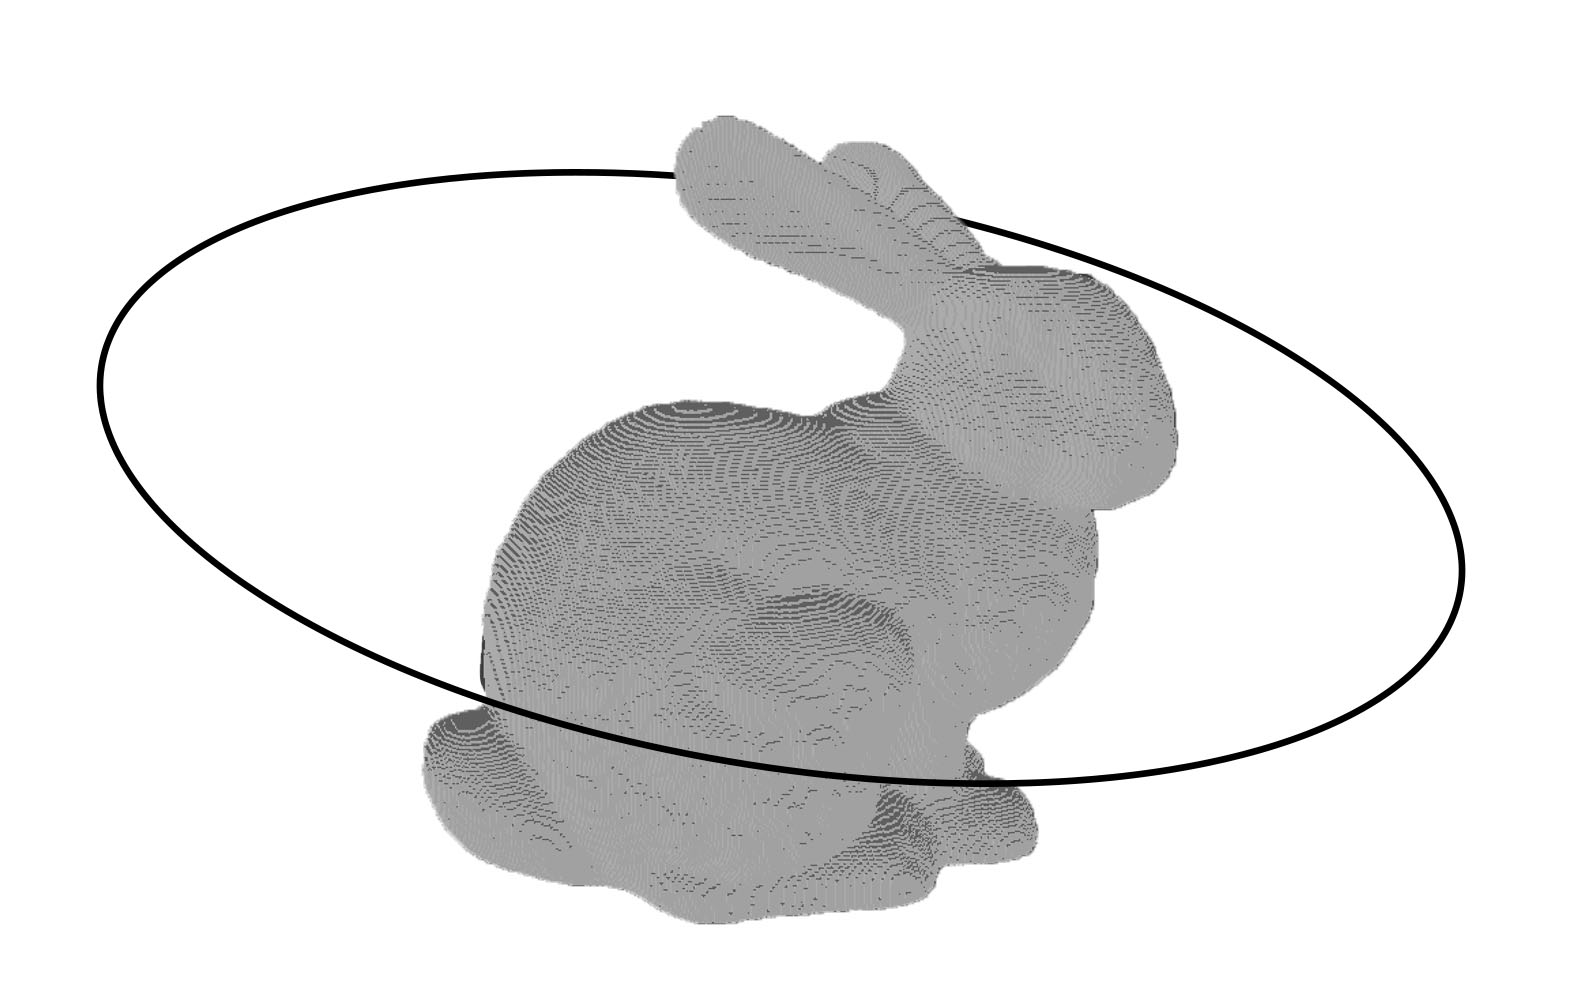
\includegraphics[width=200px]{images/graphics/test-anim-camera-path.jpg}
    \caption{During profiling, the camera is moved along an orbit around the voxel mesh, while being offset to compensate 
    for models, which behave differently when viewed from an angle. The visualization is not to scale, the models 
    are always completely visible and not culled by view frustum culling.}
    \label{fig:test-anim-camera-path}
\end{figure}



%- Compare:
%    - Model turntable rendered without OC
%    - Model turntable rendered with OC
%(   - Model turntable rendered with different OC implementation (? -> hard))
%
%
%- Criteria: 
%    - Frame time
%    - Dispatch numbers (?)
%    - Duration of depth pre-pass
%        - Draw best occluders to depth buffer
%        - Duration of depth hierarchy creation
%    - Visible cubes
%    - Visible octree nodes
%    - Triangle count
%    - Amount of best occluders
%    - CPU time
%    - GPU time
%    - Amount of overdraw (heatmap if possible)
%
%
%- Model variations:
%    - Lucy
%    - Stanford Bunny
%    - Torus (for when objects have "holes")
%    - Some large, wide scenery
%    - Sponza        -> Ehrlich sein und T
%    - ...
%
%
%- Machines:
%    - Laptop
%    - RTX 2080 Ti
%    - RTX 4090
%    - Multiple devices


\section{Culling Results}

The amount of visible voxels compared to the amount of culled voxels is one major aspect of the 
experiment and is not related to the actual performance measures. They are assumed to be the same 
for all hardware setups and are therefore only measured on the \emph{Laptop} setup. The results are 
presented below, comparing the per-octree culling with the per-meshlet culling. For the culling, the 
profiling camera animation was used to provide better average values in a more realistic environment.\\


[@TODO: Add per meshlet culling graphs into these plots!]

% --------------------------------------- LUCY 256 ---------------------------------------

\begin{figure}[h!]              % Lucy 256 Voxels Test Anim
    \begin{center}
      \begin{tikzpicture}
        \begin{axis}[
            width=\linewidth, % Scale the plot to \linewidth
            height=100px,
            xlabel={Frames},
            ylabel={Visible Voxels},
            grid,
            xmin=0,
            xmax=2392,
            ymin=100000,
            ymax=160000
          ]
          \addplot[red, no marks, solid] table[col sep=comma, x=frame, y=visible_voxels]{./plotdata/lucy_256_voxels.csv};
          \addplot[blue, dotted, no marks, domain=0:2393, samples=50] {140842};
        \end{axis}
      \end{tikzpicture}
      \caption{The amount of visible voxels over the course of the test animation shown in red. 
      The average amount of visible voxels was \emph{140,842}, which is marked as the blue dotted line.}
    \end{center}
  \end{figure}


  \begin{figure}[h!]            % Lucy 256 OT Nodes Test Anim
    \begin{center}
      \begin{tikzpicture}
        \begin{axis}[
            width=\linewidth, % Scale the plot to \linewidth
            height=100px,
            xlabel={Frames},
            ylabel={Visible Nodes},
            grid,
            xmin=0,
            xmax=2392,
            ymin=2500,
            ymax=4000
          ]
          \addplot[red, no marks, solid] table[col sep=comma, x=frame, y=visible_nodes]{./plotdata/lucy_256_nodes.csv};
          \addplot[blue, dotted, no marks, domain=0:2393, samples=50] {3460};
        \end{axis}
      \end{tikzpicture}
      \caption{The amount of visible octree nodes over the course of the test animation shown in red. 
      The average amount of visible octree nodes was \emph{3460}, which is marked as the blue dotted line.}
    \end{center}
  \end{figure}

% ----------------------------------------------------------------------------------------



% --------------------------------------- BUNNY 256 --------------------------------------

\begin{figure}[h!]              % Bunny 256 Voxels Test Anim
    \begin{center}
      \begin{tikzpicture}
        \begin{axis}[
            width=\linewidth, % Scale the plot to \linewidth
            height=100px,
            xlabel={Frames},
            ylabel={Visible Voxels},
            grid,
            xmin=0,
            xmax=1186,
            ymin=250000,
            ymax=500000
          ]
          \addplot[red, no marks, solid] table[col sep=comma, x=frame, y=visible_voxels]{./plotdata/bunny_256_voxels.csv};
          \addplot[blue, dotted, no marks, domain=0:2393, samples=50] {140842};
        \end{axis}
      \end{tikzpicture}
      \caption{The amount of visible voxels over the course of the test animation shown in red. 
      The average amount of visible voxels was \emph{140,842}, which is marked as the blue dotted line.}
    \end{center}
  \end{figure}


  \begin{figure}[h!]            % Bunny 256 OT Nodes Test Anim
    \begin{center}
      \begin{tikzpicture}
        \begin{axis}[
            width=\linewidth, % Scale the plot to \linewidth
            height=100px,
            xlabel={Frames},
            ylabel={Visible Nodes},
            grid,
            xmin=0,
            xmax=1186,
            ymin=6000,
            ymax=10000
          ]
          \addplot[red, no marks, solid] table[col sep=comma, x=frame, y=visible_nodes]{./plotdata/bunny_256_nodes.csv};
          \addplot[blue, dotted, no marks, domain=0:2393, samples=50] {3460};
        \end{axis}
      \end{tikzpicture}
      \caption{The amount of visible octree nodes over the course of the test animation shown in red. 
      The average amount of visible octree nodes was \emph{3460}, which is marked as the blue dotted line.}
    \end{center}
  \end{figure}

% ----------------------------------------------------------------------------------------





\subsection*{Laptop Setup}


\subsubsection*{Culling Effect}




















\begin{table}[h]
    \begin{tabular}{|lccccc|}
    \hline
    \multicolumn{6}{|c|}{\textbf{Scene Resolution: $256^3$}}                                                                                                                                                                                                         \\ \hline
    \multicolumn{1}{|l|}{}                          & \multicolumn{1}{|l|}{\textbf{Stanford Lucy}}  & \multicolumn{1}{l|}{\textbf{Stanford Bunny}}  & \multicolumn{1}{l|}{\textbf{Torus}}   & \multicolumn{1}{l|}{\textbf{Terrain}}     & \multicolumn{1}{l|}{\textbf{Hairball}}    \\ \hline
    \multicolumn{1}{|l|}{Total Voxel Count}         & \multicolumn{1}{c|}{331,254}                  & \multicolumn{1}{c|}{-}                        & \multicolumn{1}{c|}{-}                & \multicolumn{1}{c|}{-}                    & \multicolumn{1}{c|}{-}                    \\
    \multicolumn{1}{|l|}{Culled Voxels}             & \multicolumn{1}{c|}{207,466}                  & \multicolumn{1}{c|}{-}                        & \multicolumn{1}{c|}{-}                & \multicolumn{1}{c|}{-}                    & -                                         \\
    \multicolumn{1}{|l|}{Voxel Culling Ratio}       & \multicolumn{1}{c|}{\textbf{62,63 \%}}        & \multicolumn{1}{c|}{-}                        & \multicolumn{1}{c|}{-}                & \multicolumn{1}{c|}{-}                    & -                                         \\ \hline
    \multicolumn{1}{|l|}{Octree Nodes}              & \multicolumn{1}{c|}{6,830}                    & \multicolumn{1}{c|}{-}                        & \multicolumn{1}{c|}{-}                & \multicolumn{1}{c|}{-}                    & -                                         \\
    \multicolumn{1}{|l|}{Culled Octree Nodes}       & \multicolumn{1}{c|}{3,774}                    & \multicolumn{1}{c|}{-}                        & \multicolumn{1}{c|}{-}                & \multicolumn{1}{c|}{-}                    & -                                         \\
    \multicolumn{1}{|l|}{Octree Culling Ratio}      & \multicolumn{1}{c|}{\textbf{55,25 \%}}        & \multicolumn{1}{c|}{-}                        & \multicolumn{1}{c|}{-}                & \multicolumn{1}{c|}{-}                    & -                                         \\ \hline
    \end{tabular}
\end{table}


\subsubsection*{GPU Timings}

\begin{table}[h]
    \begin{tabular}{|lccccc|}
    \hline
    \multicolumn{6}{|c|}{\textbf{Scene Resolution: $256^3$}}                                                                                                                                                                                                         \\ \hline
    \multicolumn{1}{|l|}{}                          & \multicolumn{1}{l|}{\textbf{Stanford Lucy}}   & \multicolumn{1}{l|}{\textbf{Stanford Bunny}}  & \multicolumn{1}{l|}{\textbf{Torus}}   & \multicolumn{1}{l|}{\textbf{Terrain}}     & \multicolumn{1}{l|}{\textbf{Hairball}}    \\ \hline
    \multicolumn{1}{|l|}{Overall GPU Time}          & \multicolumn{1}{c|}{2.3009 ms}                & \multicolumn{1}{c|}{-}                        & \multicolumn{1}{c|}{-}                & \multicolumn{1}{c|}{-}                    & \multicolumn{1}{c|}{-}                    \\
    \multicolumn{1}{|l|}{Depth Pre-Pass}            & \multicolumn{1}{c|}{402.7 us}                 & \multicolumn{1}{c|}{-}                        & \multicolumn{1}{c|}{-}                & \multicolumn{1}{c|}{-}                    & -                                         \\
    \multicolumn{1}{|l|}{Dispatch Mesh (Draw)}      & \multicolumn{1}{c|}{1.75 ms}                  & \multicolumn{1}{c|}{-}                        & \multicolumn{1}{c|}{-}                & \multicolumn{1}{c|}{-}                    & -                                         \\ \hline
    \end{tabular}
\end{table}





\section{Per-Meshlet Culling Results}

\subsection*{Laptop Setup}

\subsubsection*{Culling Effect}

\begin{table}[h]
    \begin{tabular}{|lccccc|}
    \hline
    \multicolumn{6}{|c|}{\textbf{Scene Resolution: $256^3$}}                                                                                                                                                                                                         \\ \hline
    \multicolumn{1}{|l|}{}                          & \multicolumn{1}{|l|}{\textbf{Stanford Lucy}}  & \multicolumn{1}{l|}{\textbf{Stanford Bunny}}  & \multicolumn{1}{l|}{\textbf{Torus}}   & \multicolumn{1}{l|}{\textbf{Terrain}}     & \multicolumn{1}{l|}{\textbf{Hairball}}    \\ \hline
    \multicolumn{1}{|l|}{Total Voxel Count}         & \multicolumn{1}{c|}{331,254}                  & \multicolumn{1}{c|}{-}                        & \multicolumn{1}{c|}{-}                & \multicolumn{1}{c|}{-}                    & \multicolumn{1}{c|}{-}                    \\
    \multicolumn{1}{|l|}{Culled Voxels}             & \multicolumn{1}{c|}{257,961}                  & \multicolumn{1}{c|}{-}                        & \multicolumn{1}{c|}{-}                & \multicolumn{1}{c|}{-}                    & -                                         \\
    \multicolumn{1}{|l|}{Voxel Culling Ratio}       & \multicolumn{1}{c|}{\textbf{77,87 \%}}        & \multicolumn{1}{c|}{-}                        & \multicolumn{1}{c|}{-}                & \multicolumn{1}{c|}{-}                    & -                                         \\ \hline
    \multicolumn{1}{|l|}{Octree Nodes}              & \multicolumn{1}{c|}{6,830}                    & \multicolumn{1}{c|}{-}                        & \multicolumn{1}{c|}{-}                & \multicolumn{1}{c|}{-}                    & -                                         \\
    \multicolumn{1}{|l|}{Culled Octree Nodes}       & \multicolumn{1}{c|}{4,329}                    & \multicolumn{1}{c|}{-}                        & \multicolumn{1}{c|}{-}                & \multicolumn{1}{c|}{-}                    & -                                         \\
    \multicolumn{1}{|l|}{Octree Culling Ratio}      & \multicolumn{1}{c|}{\textbf{63,38 \%}}        & \multicolumn{1}{c|}{-}                        & \multicolumn{1}{c|}{-}                & \multicolumn{1}{c|}{-}                    & -                                         \\ \hline
    \end{tabular}
\end{table}


\subsubsection*{GPU Timings}

\begin{table}[h]
    \begin{tabular}{|lccccc|}
    \hline
    \multicolumn{6}{|c|}{\textbf{Scene Resolution: 256\textasciicircum{}3}}                                                                                                                                                                                                         \\ \hline
    \multicolumn{1}{|l|}{}                          & \multicolumn{1}{l|}{\textbf{Stanford Lucy}}   & \multicolumn{1}{l|}{\textbf{Stanford Bunny}}  & \multicolumn{1}{l|}{\textbf{Torus}}   & \multicolumn{1}{l|}{\textbf{Terrain}}     & \multicolumn{1}{l|}{\textbf{Hairball}}    \\ \hline
    \multicolumn{1}{|l|}{Overall GPU Time}          & \multicolumn{1}{c|}{1.7162 ms}                & \multicolumn{1}{c|}{-}                        & \multicolumn{1}{c|}{-}                & \multicolumn{1}{c|}{-}                    & \multicolumn{1}{c|}{-}                    \\
    \multicolumn{1}{|l|}{Depth Pre-Pass}            & \multicolumn{1}{c|}{388.3 us}                 & \multicolumn{1}{c|}{-}                        & \multicolumn{1}{c|}{-}                & \multicolumn{1}{c|}{-}                    & -                                         \\
    \multicolumn{1}{|l|}{Dispatch Mesh (Draw)}      & \multicolumn{1}{c|}{1.19 ms}                  & \multicolumn{1}{c|}{-}                        & \multicolumn{1}{c|}{-}                & \multicolumn{1}{c|}{-}                    & -                                         \\ \hline
    \end{tabular}
\end{table}







- Results of the case study

- Table for drawn vs occluded voxels in numbers and percent
- Table for Execution times (full frame, prepass, draw, ...)
- Table for triangles drawn vs. culled 
- Table for 
